\chapter{Konečné automaty}\label{chap:automaty}
V~této kapitole se budeme věnovat základům \emph{teorie automatů}. Konečné automaty jsou jednoduché abstraktní stroje,~které zpracovávají vstupní slovo znak po znaku a~na konci rozhodnou,~zda jej přijmou,~nebo odmítnou. Množiny přijímaných slov tvoří tzv. \emph{formální jazyky}.

Nejdříve si zavedeme potřebné operace nad slovy a~jazyky. Poté se podíváme na deterministické a~nedeterministické konečné automaty,~regulární výrazy a~formální gramatiky. Ukáže se,~že konečné automaty,~regulární výrazy a~regulární gramatiky jsou tři různé způsoby popisu stejné třídy jazyků. Později tuto teorii využijeme při lexikální analýze v~kapitole \smartref{\showrefs}{chap:kompilatory}{o~kompilátorech}.

\section{Úvod}\label{sec:uvod}

Konečné (stavové) automaty představují abstraktní stroje reprezentující určitý výpočet nebo algoritmus. Z reálného světa můžeme za stavový automat považovat např. obyčejný vypínač, viz obrázek \ref{fig:vypinac}.
\begin{figure}[h]
    \begin{center}
        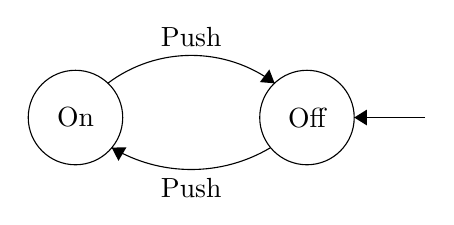
\begin{tikzpicture}[scale=0.2]
        \tikzstyle{every node}+=[inner sep=0pt]
        \draw [black] (29,-28.9) circle (3);
        \draw (29,-28.9) node {On};
        \draw [black] (43.7,-28.9) circle (3);
        \draw (43.7,-28.9) node {Off};
        \draw [black] (31.047,-26.727) arc (126.9692:53.0308:8.818);
        \fill [black] (41.65,-26.73) -- (41.31,-25.85) -- (40.71,-26.65);
        \draw (36.35,-24.45) node [above] {Push};
        \draw [black] (41.399,-30.806) arc (-59.10767:-120.89233:9.833);
        \fill [black] (31.3,-30.81) -- (31.73,-31.65) -- (32.24,-30.79);
        \draw (36.35,-32.7) node [below] {Push};
        \draw [black] (51.2,-28.9) -- (46.7,-28.9);
        \fill [black] (46.7,-28.9) -- (47.5,-29.4) -- (47.5,-28.4);
        \end{tikzpicture}
    \end{center}
    \caption{Schéma automatu pro vypínač.}
    \label{fig:vypinac}
\end{figure}
Příkladem praktického použití návrhu automatů je tzv. \emph{lexikální analýza}, kterou se budeme zabývat v kapitole~\smartref[][ v sekci \dots]{true}{chap:kompilatory}{o kompilátorech}. Na obrázku \ref{fig:automat-then} je vidět příklad konečného automatu rozpoznávající slovo \textit{then}.
\begin{figure}[h]
    \begin{center}
        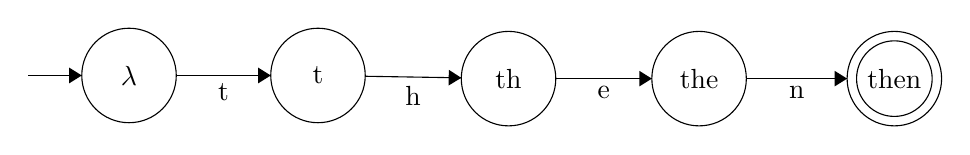
\begin{tikzpicture}[scale=0.2]
        \tikzstyle{every node}+=[inner sep=0pt]
        \draw [black] (17.7,-28.6) circle (3);
        \draw (17.7,-28.6) node {$\lambda$};
        \draw [black] (29.7,-28.6) circle (3);
        \draw (29.7,-28.6) node {t};
        \draw [black] (41.8,-28.8) circle (3);
        \draw (41.8,-28.8) node {th};
        \draw [black] (53.9,-28.8) circle (3);
        \draw (53.9,-28.8) node {the};
        \draw [black] (66.3,-28.8) circle (3);
        \draw (66.3,-28.8) node {then};
        \draw [black] (66.3,-28.8) circle (2.4);
        \draw [black] (11.3,-28.6) -- (14.7,-28.6);
        \fill [black] (14.7,-28.6) -- (13.9,-28.1) -- (13.9,-29.1);
        \draw [black] (20.7,-28.6) -- (26.7,-28.6);
        \fill [black] (26.7,-28.6) -- (25.9,-28.1) -- (25.9,-29.1);
        \draw (23.7,-29.1) node [below] {t};
        \draw [black] (32.7,-28.65) -- (38.8,-28.75);
        \fill [black] (38.8,-28.75) -- (38.01,-28.24) -- (37.99,-29.24);
        \draw (35.74,-29.22) node [below] {h};
        \draw [black] (44.8,-28.8) -- (50.9,-28.8);
        \fill [black] (50.9,-28.8) -- (50.1,-28.3) -- (50.1,-29.3);
        \draw (47.85,-29.3) node [below] {e};
        \draw [black] (56.9,-28.8) -- (63.3,-28.8);
        \fill [black] (63.3,-28.8) -- (62.5,-28.3) -- (62.5,-29.3);
        \draw (60.1,-29.3) node [below] {n};
        \end{tikzpicture}
        \end{center}
    \caption{Schéma automatu rozpoznávající slovo \texttt{then}.}
    \label{fig:automat-then}
\end{figure}

Jak tedy vlastně konečné automaty fungují? Vstup je reprezentován určitou \textbf{konečnou posloupností znaků}, tedy nějakým řetězcem neboli tzv. \textbf{slovem}, které daný automat zpracováva postupně po jednotlivých znacích. Na konci výpočtu vydá automat odpověď, zda vstup \textbf{přijal}, či \textbf{nepřijal} (viz obrázek \ref{fig:konecny-automat}).
\begin{figure}[h]
    \centering
    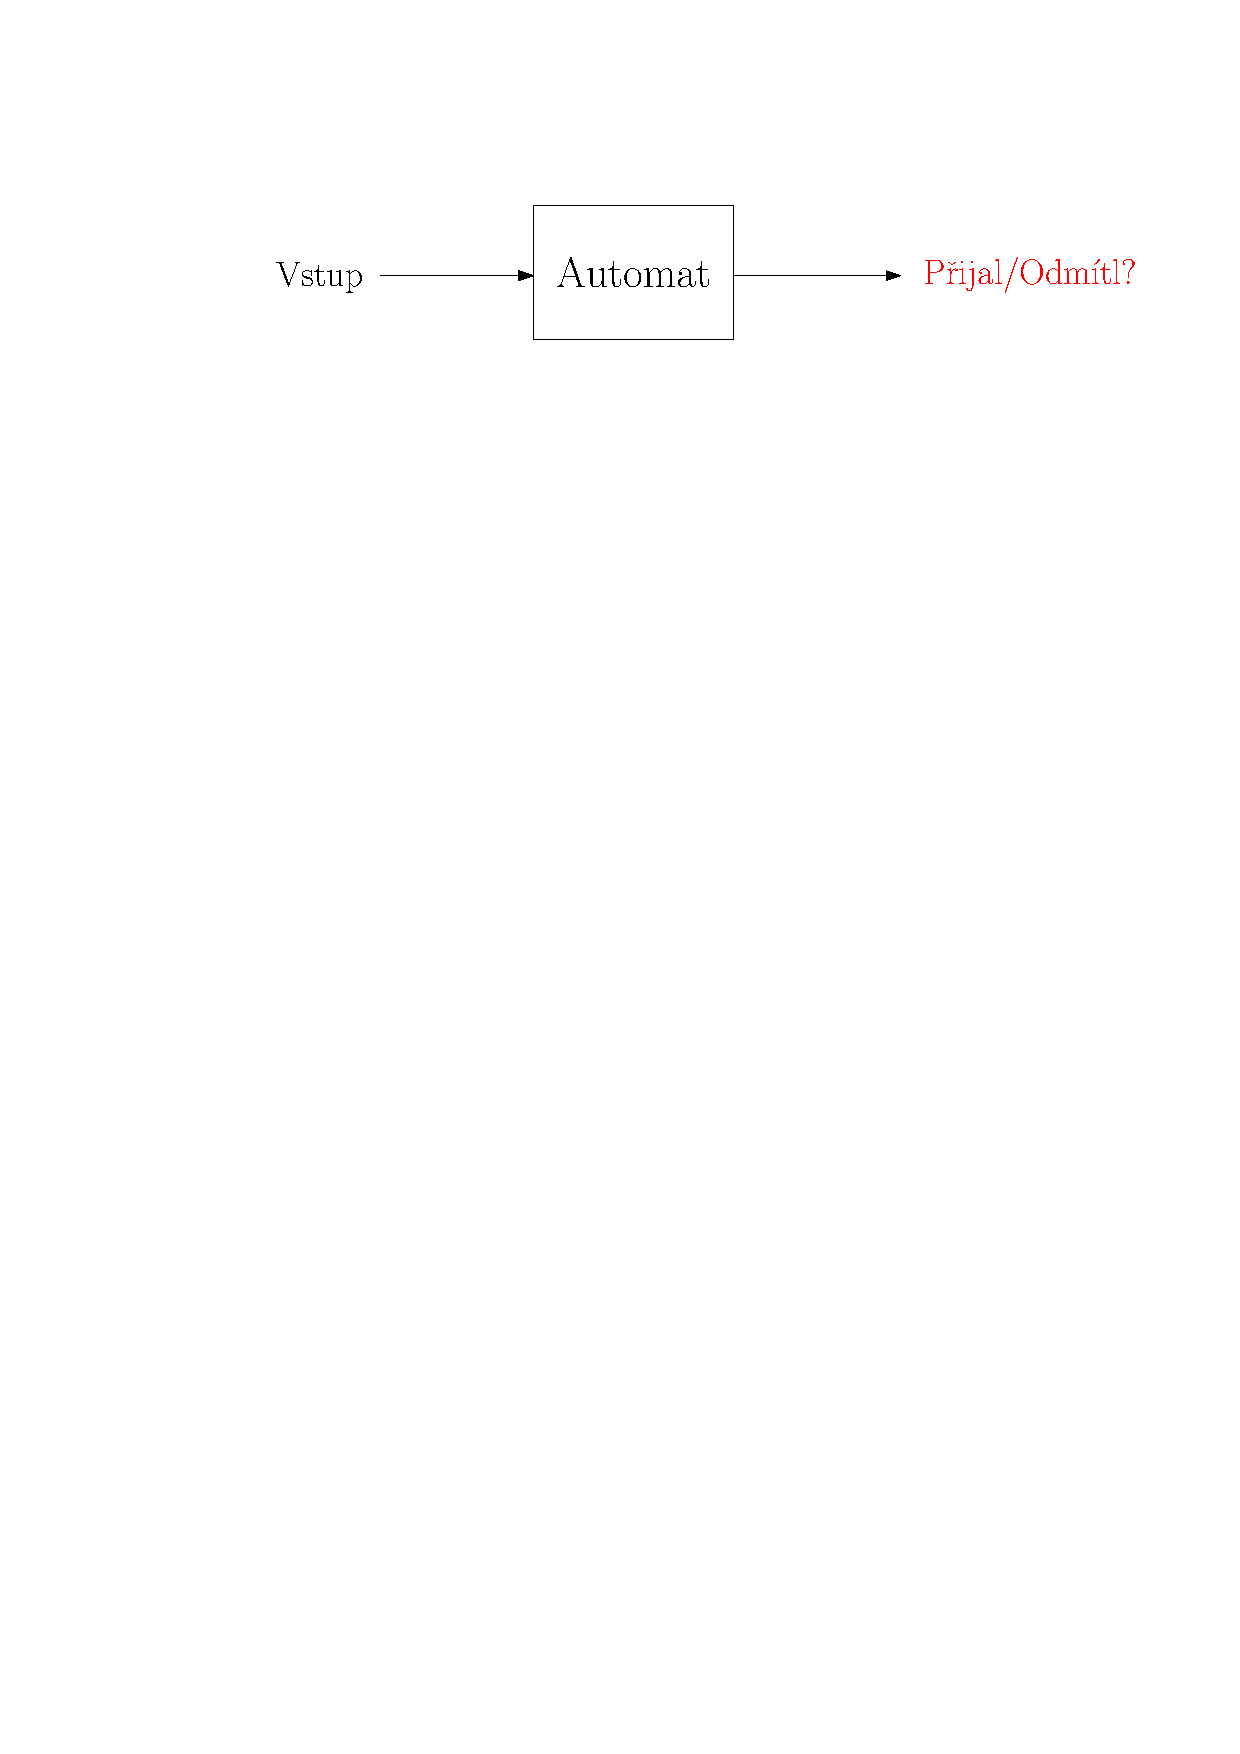
\includegraphics[scale=.7]{03-automaty/images/ch03_konecny-automat.pdf}
    \caption{Zjednodušené schéma konečného automatu.}
    \label{fig:konecny-automat}
\end{figure}
\section{Formální jazyky}\label{sec:jazyky}

Nyní, když jsme si vysvětlili základy konečných automatů a~jejich roli ve zpracovávání formálních jazyků, můžeme se hlouběji ponořit do problematiky formálních jazyků samotných. Tyto jazyky jsou totiž základem pro popis množin řetězců a~jsou klíčové pro definování toho, co automaty rozpoznávají.

Formální jazyky lze chápat jako abstraktní systémy pro popis pravidel, podle kterých jsou vytvářeny řetězce symbolů. Jsou zásadní nejen pro teorii automatů, ale také pro návrh programovacích jazyků a~kompilátorů. V~následujících částech se zaměříme na různé typy gramatik, které jsou základem pro definici formálních jazyků, a~ukážeme si, jak konečné automaty mohou tyto jazyky rozpoznávat a~zpracovávat.

Pro začátek si (jako vždy) uvedeme definice některých základních pojmů.
\begin{definition}
    Máme neprázdnou množinu znaků $\Sigma$, tzv. \textbf{abecedu}.
    \begin{itemize}
        \item \textbf{Slovo (řetězec)} je libovolná konečná posloupnost znaků ze $\Sigma$.
        \item \textbf{Prázdné slovo} je slovo neobsahující žádné znaky\footnote{Symbol $\lambda$ zde představuje speciální znak zastupující prázdné slovo. Neuvažujeme jej tedy jako součást abecedy $\Sigma$, tzn. $\lambda\notin\Sigma$.}, značíme $\lambda$.
        \item \textbf{Množina všech slov v abecedě $\Sigma$} se značí $\Sigma^*$.
        \item \textbf{Jazyk} je libovolná podmnožina slov $L\subseteq\Sigma$. Říkáme, že jazyk $L$ je \emph{nad abecedou $\Sigma$} (viz obrázek \ref{fig:jazyk}).
        \begin{figure}[h]
            \centering
            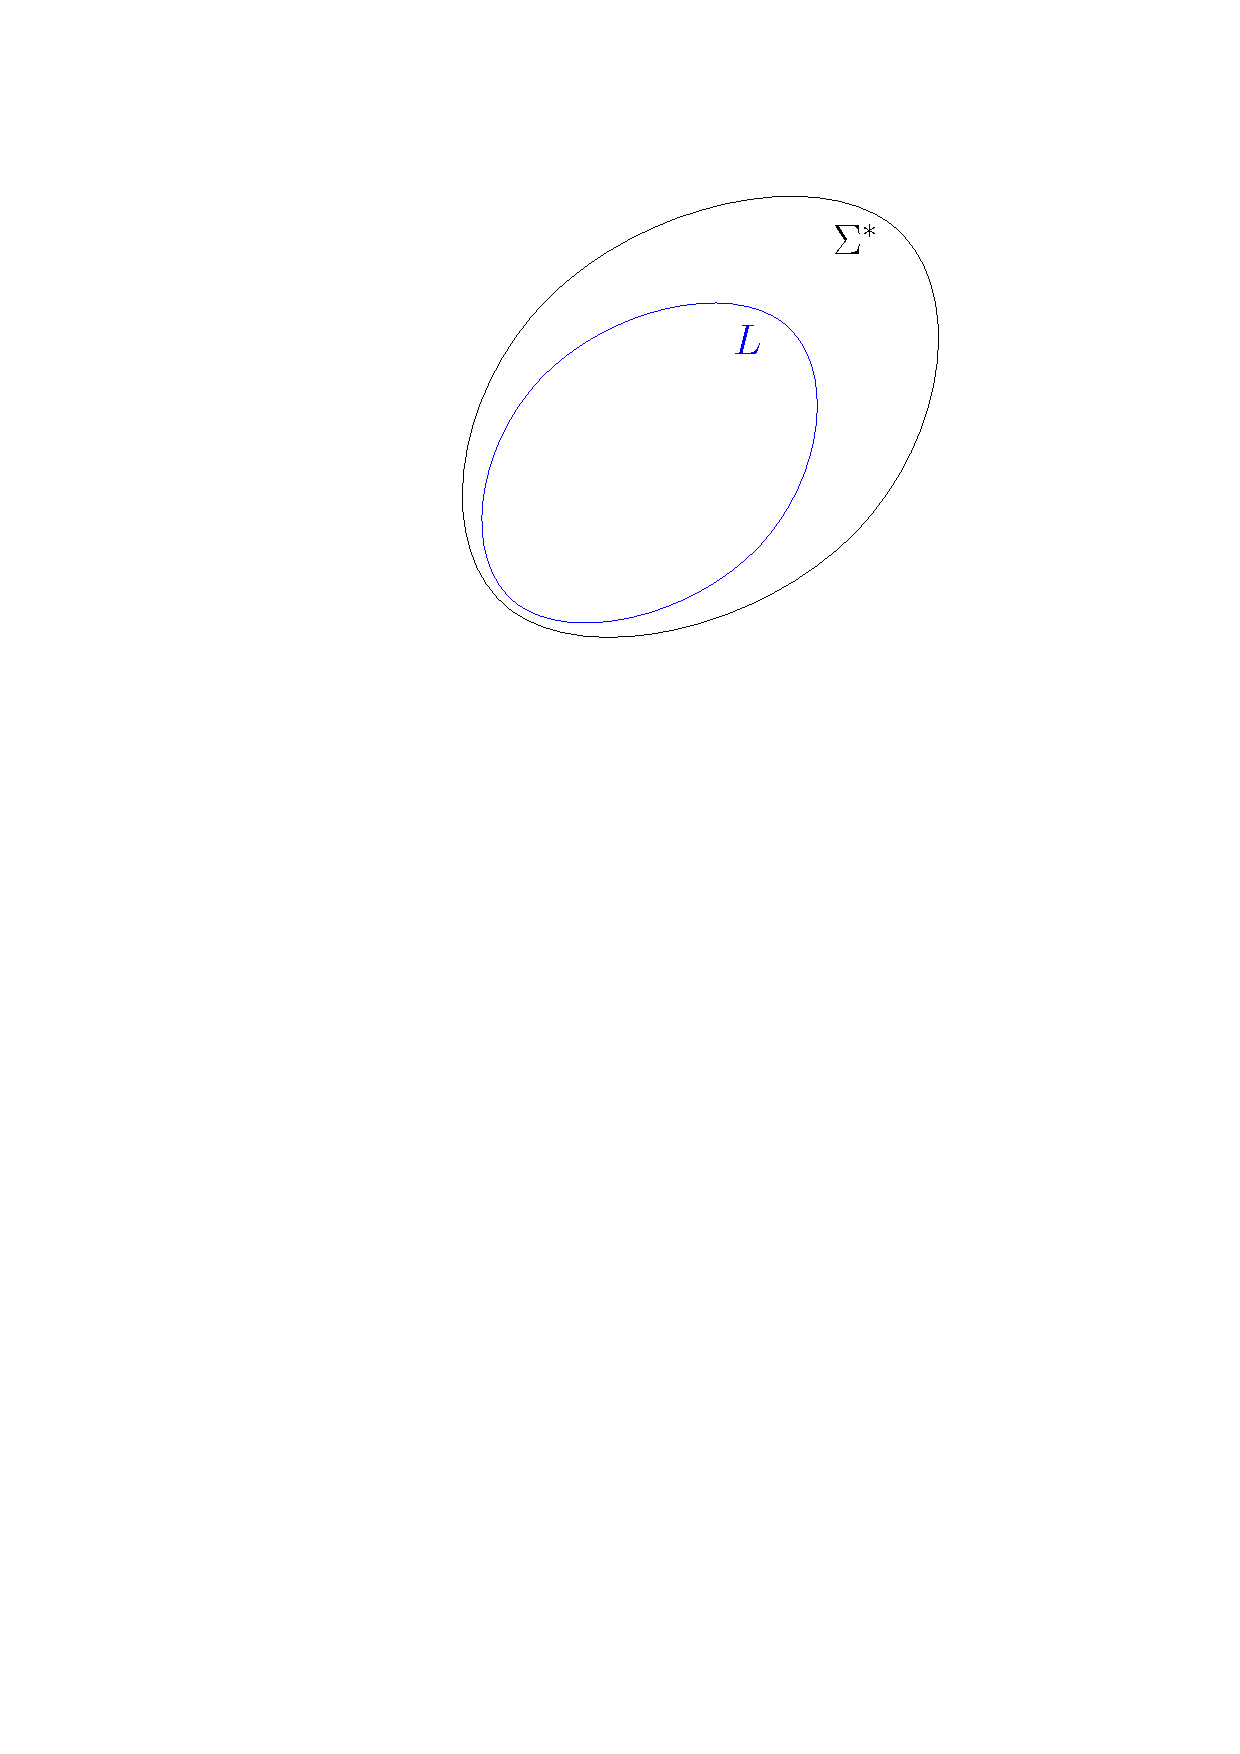
\includegraphics[scale=.7]{03-automaty/images/ch03_jazyk.pdf}
            \caption{Obecný jazyk $L$ nad abecedou $\Sigma$.}
            \label{fig:jazyk}
        \end{figure}
        \item \textbf{Délka slova} $w$ (tzn. počet znaků) se značí $|w|$.
        \item \textbf{Konkantenace} slov $u,v\in\Sigma^*$, kde $u=u_1u_2\dots u_n$ a $v=v_1v_2\dots v_m$ je slovo
        \[uv=u_1u_2\dots u_nv_1v_2\dots v_m.\]
        \item \textbf{$n$-tá mocnina} slova $u\in\Sigma^*$ je slovo
        \[u^n=\underbrace{uu\dots u}_{\text{$n$-krát}},\]
        kde $n\in\N_0$. Speciálně $u^0=\lambda$.
    \end{itemize}
\end{definition}
Podívejme se na jednoduchý příklad.
\begin{example}
    Mějme dvouznakovou abecedu $\Sigma=\set{a,b}$.
    \begin{itemize}
        \item Např. slovem v takto zadané abecedě $\Sigma$ je $w=abba$. Tzn. $|w|=4$.
        \item Množina všech slov\footnote{Je pochopiltené, že tato množina je nekonečná (délka slov není nijak omezená).} $\Sigma^*=\set{\lambda,a,b,aa,ab,ba,bb,aaa,aab,aba,\dots}$.
        \item Jednoduchý příklad jazyka nad abecedou $\Sigma$ je $L_1=\Sigma^*$, tedy všechna možná slova sestávající ze znaků $a,b$.
        \item Dalším příkladem může být např. jazyk $L_2=\set{w\in\Sigma^*\mid |w|\leqslant 2}$. Jazyk $L_2$ tedy obsahuje všechna slova délky nejvýše $2$, tj.
        \[L_2=\set{\lambda,a,b,aa,ab,ba,bb}.\]
        \item Pátá mocnina slova $w=abba$:
        \[w^5=abbaabbaabbaabbaabba.\]
        \item Konkantenace slov $u=aabb$ a $v=bbaa$
        \[uv=aabbbbaa.\]
    \end{itemize}
\end{example}

Jazyky nejsou v matematickém pojetí nic jiné než množiny objektů, tedy v tomto případě slov.
\begin{example}
    Další příklady jazyků:
    \begin{itemize}
        \item Jazyk $U=\set{w\in\Sigma^*\mid w\subseteq\set{X,Y}^*}$ obsahující všechna \emph{slova sestávající pouze z velkých písmen} nad abecedou $\Sigma=\set{x,y,X,Y}$.
        \item Jazyk $N=\set{u\in\Lambda^*\mid |u|\geqslant 1}$ obsahující všechna \emph{neprázdná slova} nad obecnou abecedou $\Lambda$ (může být jakákoliv).
        \item Jazyk $Z=\set{0^n1^n\mid n\in\N}$ nad abecedou $\Omega=\set{0,1}$.
    \end{itemize}
\end{example}
\section{Deterministické konečné automaty}\label{sec:det-automaty}

Již jsme si představili jazyky jakožto prostředek pro reprezentaci vstupů pro konečné automaty. Stále jsme si ovšem neřekli, co to ten automat vlastně je. Podobně jako v definici grafu, kdy máme uspořádanou dvojici vrcholů a hran, i zde bude myšlenka velice podobná.
\begin{definition}[Deterministický končný automat]
    \emph{Deterministický konečný automat} je uspořádaná pětice $A=(Q,\Sigma,\delta,q_0,F)$, kde
    \begin{itemize}
        \item $Q$ je konečná \emph{množina stavů},
        \item $\Sigma$ je abeceda, z níž sestávají slova na vstupu,
        \item $\delta$ je tzv. \emph{přechodová funkce} $Q\times\Sigma\rightarrow Q$ udávající přechody mezi stavy,
        \item $q_0\in Q$ je \emph{počáteční stav} automatu
        \item a $F\subseteq Q$ je \emph{množina přijímajících stavů}.
    \end{itemize}
\end{definition}
Automaty zakreslujeme pomocí stavového diagramu (formálně orientovaného grafu), přičemž
\begin{itemize}
    \item \emph{vrcholy} jsou jednotlivé stavy automatu (dvojitý kruh značí přijímající stav a do počátečního stavu vede šipka ``odnikud'')
    \item a \emph{šipky} reprezentují přechody mezi stavy.
\end{itemize}
Na začátku výpočtu dostane automat na vstupu slovo $w\in\Sigma^*$, které čte znak po znaku (zleva doprava). Začínáme v počátečním stavu $q_0$, přičemž vždy podle následujícího čteného znaku se automat přesouvá do nového stavu. Přechodová funkce $\delta:Q\times\Sigma\rightarrow Q$ nám udává pro každou dvojici $(q,a)$, kde $q$ je stav, v němž se automat nachází a $a$ je aktuálně čtený znak, do jakého stavu se má automat přesunout. Pokud na konci čtení slova $w$ skončí výpočet v jednom z přijímajících stavů, pak automat slovo přijímá. V opačném případě, kdy výpočet neskončí v přijímajícím stavu nebo přechod pro určitý znak z určitéhoi stavu není definovaný, pak výpočet končí a automat slovo nepřijímá.
\begin{example}
    Máme automat $A=(Q,\Sigma,\delta,q_0,F)$, kde
    \begin{itemize}
        \item $Q=\set{q_0,q_1,q_2}$,
        \item $q_0$ je počáteční stav,
        \item $F=\set{q_2}$,
        \item $\Sigma=\set{0,1}$,
        \item Přechodová funkce $\delta$ (viz tabulka \ref{tab:prechodova-funkce-A}):
        \begin{itemize}
            \item $\delta(q_0,0)=q_1$,
            \item $\delta(q_0,1)=q_2$,
            \item $\delta(q_0,0)=q_2$,
            \item $\delta(q_0,1)=q_2$.
        \end{itemize}
    \end{itemize}
    Schéma automatu lze vidět na obrázku \ref{fig:automat-A} níže.
    \begin{figure}[h]
        \centering
        \centering
        \begin{center}
            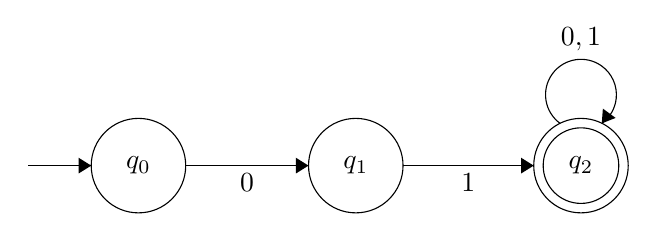
\begin{tikzpicture}[scale=0.2]
            \tikzstyle{every node}+=[inner sep=0pt]
            \draw [black] (18.8,-30.5) circle (3);
            \draw (18.8,-30.5) node {$q_0$};
            \draw [black] (32.6,-30.5) circle (3);
            \draw (32.6,-30.5) node {$q_1$};
            \draw [black] (46.9,-30.5) circle (3);
            \draw (46.9,-30.5) node {$q_2$};
            \draw [black] (46.9,-30.5) circle (2.4);
            \draw [black] (21.8,-30.5) -- (29.6,-30.5);
            \fill [black] (29.6,-30.5) -- (28.8,-30) -- (28.8,-31);
            \draw (25.7,-31) node [below] {$0$};
            \draw [black] (35.6,-30.5) -- (43.9,-30.5);
            \fill [black] (43.9,-30.5) -- (43.1,-30) -- (43.1,-31);
            \draw (39.75,-31) node [below] {$1$};
            \draw [black] (45.577,-27.82) arc (234:-54:2.25);
            \draw (46.9,-23.25) node [above] {$0,1$};
            \fill [black] (48.22,-27.82) -- (49.1,-27.47) -- (48.29,-26.88);
            \draw [black] (11.8,-30.5) -- (15.8,-30.5);
            \fill [black] (15.8,-30.5) -- (15,-30) -- (15,-31);
            \end{tikzpicture}
        \end{center}
        \caption{Schéma automatu $A$ a tabulka přechodové funkce $\delta$}
        \label{fig:automat-A}
    \end{figure}
    \begin{table}[h]
        \centering
        \begin{tabular}{c|cc}
        & $0$           & $1$           \\ \hline
        $q_0$      & $q_1$        & -- \\
        $q_1$      & -- & $q_2$        \\
        $q_2$      & $q_2$        & $q_2$        \\
        \end{tabular}
        \caption{Tabulka přechodové funkce $\delta$ automatu $A$}
        \label{tab:prechodova-funkce-A}
    \end{table}
\end{example}
\section{Nedeterministické konečné automaty}\label{sec:nedet-automaty}

U~deterministického automatu vede pro daný stav a~znak nejvýše jeden přechod. Někdy je však návrh mnohem jednodušší,~když automatu dovolíme několik možností a~představíme si,~že vyzkouší všechny paralelně.

\begin{definition}[Potenční množina]
    Nechť $M$ je množina. \emph{Potenční množinou} množiny $M$ nazveme množinu všech jejích podmnožin. Značíme ji
    \[
        \powset{M}=\set{N:N\subseteq M}.
    \]
    Například pro $M=\set{q_0,q_1}$ dostaneme
    \[
        \powset{M}=\set{\emptyset,\set{q_0},\set{q_1},\set{q_0,q_1}}.
    \]
\end{definition}

\begin{definition}[Nedeterministický konečný automat]
    \emph{Nedeterministický konečný automat} (zkráceně NFA) je pětice
    \[A=(Q,\Sigma,\delta,q_0,F),\]
    kde $Q$,~$\Sigma$,~$q_0$ a~$F$ mají stejný význam jako u~DFA a
    \[\delta:Q\times\Sigma\to\powset{Q}\]
    přiřazuje dvojici stavu a~znaku množinu možných následujících stavů.
\end{definition}

Přečte-li NFA ve stavu $q$ znak $a$,~výpočet se rozvětví do všech stavů z~$\delta(q,a)$. Je-li tato množina prázdná,~daná větev zanikne. Automat přijme vstupní slovo právě tehdy,~když \emph{alespoň jedna} větev po přečtení celého slova skončí v~přijímajícím stavu.

\begin{example}[Slova obsahující podslovo $101$]\label{ex:nfa-101}
    Počáteční stav $q_0$ zpracovává libovolný začátek slova. Při každé jedničce může automat zároveň \uv{uhádnout},~že právě začalo hledané podslovo,~a~spustit novou větev ve stavu $q_1$.
    \begin{figure}[h]
        \centering
        \begin{tikzpicture}
    \initialstate{q0}{(0,0)}{$q_0$}{(-1.2,0)}{180}
    \state{q1}{(2.4,0)}{$q_1$}
    \state{q2}{(4.8,0)}{$q_2$}
    \acceptingstate{q3}{(7.2,0)}{$q_3$}
    \transitionarrow[loop above]{q0}{above}{$0,1$}{q0}
    \transitionarrow{q0}{above}{$1$}{q1}
    \transitionarrow{q1}{above}{$0$}{q2}
    \transitionarrow{q2}{above}{$1$}{q3}
    \transitionarrow[loop above]{q3}{above}{$0,1$}{q3}
\end{tikzpicture}

        \caption{NFA přijímající právě slova obsahující podslovo $101$.}
        \label{fig:nfa-101}
    \end{figure}
    Pro slovo $01101$ vznikne přijímající větev,~která po posledních třech znacích projde stavy $q_1,q_2,q_3$.
\end{example}

\begin{example}[Třetí znak od konce je $1$]\label{ex:nfa-treti-od-konce}
    NFA může při každé přečtené jedničce odhadnout,~že do konce zbývají právě dva znaky. Pak už pouze odpočítá dva další přechody.
    \begin{figure}[h]
        \centering
        \begin{tikzpicture}
    \initialstate{q0}{(0,0)}{$q_0$}{(-1.2,0)}{180}
    \state{q1}{(2.5,0)}{$q_1$}
    \state{q2}{(5,0)}{$q_2$}
    \acceptingstate{q3}{(7.5,0)}{$q_3$}
    \transitionarrow[loop above]{q0}{above}{$0,1$}{q0}
    \transitionarrow{q0}{above}{$1$}{q1}
    \transitionarrow{q1}{above}{$0,1$}{q2}
    \transitionarrow{q2}{above}{$0,1$}{q3}
\end{tikzpicture}

        \caption{NFA pro jazyk slov,~jejichž třetí znak od konce je $1$.}
        \label{fig:nfa-treti-od-konce}
    \end{figure}
    Tento automat má jen čtyři stavy. Ekvivalentní DFA si musí pamatovat všechny možné konce délky tři a~potřebuje osm stavů.
\end{example}

\begin{example}[Jednoduchý zápis desetinného čísla]
    Automat na obrázku \ref{fig:automat-desetinne} přijímá neprázdný blok číslic a~případně desetinnou tečku následovanou dalším neprázdným blokem číslic. Přijme tedy \texttt{17} a~\texttt{17.25},~ale odmítne \texttt{.25},~\texttt{17.} i~\texttt{1.2.3}.
    \begin{figure}[h]
        \centering
        \begin{tikzpicture}
    \initialstate{s}{(0,0)}{$s$}{(-1.2,0)}{180}
    \acceptingstate{i}{(2.5,0)}{$q_i$}
    \state{dot}{(5,0)}{$q_t$}
    \acceptingstate{f}{(7.5,0)}{$q_f$}
    \transitionarrow{s}{above}{$0,\dots,9$}{i}
    \transitionarrow[loop above]{i}{above}{$0,\dots,9$}{i}
    \transitionarrow{i}{above}{\texttt{.}}{dot}
    \transitionarrow{dot}{above}{$0,\dots,9$}{f}
    \transitionarrow[loop above]{f}{above}{$0,\dots,9$}{f}
\end{tikzpicture}

        \caption{Konečný automat pro jednoduchý zápis nezáporného desetinného čísla.}
        \label{fig:automat-desetinne}
    \end{figure}
\end{example}

\subsection{Vztah DFA a~NFA}

Nedeterminismus sice může výrazně zjednodušit zápis automatu,~ale nerozšíří množinu jazyků,~které konečné automaty dokážou přijímat.

\begin{theorem}[Podmnožinová konstrukce]\label{thm:subset-construction}
    Ke každému NFA $A$ existuje DFA $B$ takový,~že $L(A)=L(B)$.
\end{theorem}
\begin{proof}
    Mějme NFA $A=(Q,\Sigma,\delta,q_0,F)$. Jeden stav nového DFA bude popisovat celou množinu stavů,~v~nichž se NFA může po přečtení stejného začátku slova nacházet. Položíme tedy
    \[B=(\powset{Q},\Sigma,\delta',\set{q_0},F'),\]
    kde
    \[\delta'(S,a)=\bigcup_{q\in S}\delta(q,a)\]
    a~množina $S\subseteq Q$ je přijímajícím stavem právě tehdy,~když $S\cap F\neq\emptyset$.

    Indukcí podle délky přečteného slova dostaneme,~že stav DFA $B$ je vždy přesně množinou všech stavů,~ve kterých mohou být jednotlivé větve NFA $A$. DFA proto přijme právě tehdy,~když alespoň jedna větev NFA skončí v~$F$.
\end{proof}

Každý DFA je zároveň NFA,~jen všechny množiny $\delta(q,a)$ mají nejvýše jeden prvek. Oba modely tedy přijímají stejné jazyky. Cena za odstranění nedeterminismu může být vysoká: NFA s~$n$ stavy může podmnožinovou konstrukcí vytvořit DFA až s~$2^n$ stavy.

\subsection{Přechody bez čtení znaku}

Pro důkaz Kleeneho věty se nám bude hodit ještě drobné technické rozšíření.

\begin{definition}[$\lambda$-NFA]
    \emph{$\lambda$-NFA} je NFA s~přechodovou funkcí
    \[
        \delta:Q\times(\Sigma\cup\set{\lambda})\to\powset{Q},
    \]
    který smí navíc použít přechod označený $\lambda$. Při takovém přechodu změní stav,~aniž by přečetl znak vstupu.
\end{definition}

Takový automat stále nepřijímá nic navíc. Pro množinu stavů $S$ označme $E(S)$ množinu všech stavů dosažitelných ze $S$ pouze pomocí nulového nebo více $\lambda$-přechodů. Obyčejný NFA sestrojíme tak,~že pro každý stav $q$ a~znak $a$ položíme
\[\delta'(q,a)=E\left(\bigcup_{r\in E(\set{q})}\delta(r,a)\right)\]
a~stav $q$ prohlásíme za přijímající,~pokud $E(\set{q})\cap F\neq\emptyset$. Nový automat před každým znakem i~po něm provede předem všechny možné $\lambda$-přechody,~takže přijímá tentýž jazyk.

\subsection{Regulární jazyky}

\begin{definition}[Regulární jazyk]
    Jazyk $L$ nazveme \emph{regulární},~pokud existuje DFA $A$ takový,~že $L=L(A)$.
\end{definition}

Podle věty \ref{thm:subset-construction} můžeme v~definici stejně dobře použít NFA nebo $\lambda$-NFA. Ne každý jazyk je však regulární.

\begin{theorem}\label{thm:leq-neregular}
    Jazyk
    \[L_{\mathrm{eq}}=\set{w\in\set{0,1}^*:|w|_0=|w|_1}\]
    není regulární.
\end{theorem}
\begin{proof}
    Předpokládejme pro spor,~že existuje DFA $A$ s~$m$ stavy a~$L(A)=L_{\mathrm{eq}}$. Uvažujme $m+1$ slov
    \[\lambda,0,00,\dots,0^m.\]
    Automat má jen $m$ stavů,~takže po přečtení dvou různých slov $0^i$ a~$0^j$,~kde $0\leqslant i<j\leqslant m$,~musí být ve stejném stavu.

    Nyní k~oběma slovům připojme stejný konec $1^i$. Automat z~téhož stavu čte tentýž zbytek,~a~proto buď přijme obě slova,~nebo obě odmítne. Jenže
    \[0^i1^i\in L_{\mathrm{eq}},\qquad 0^j1^i\notin L_{\mathrm{eq}}.\]
    Automat by je musel rozlišit. Dostáváme spor.
\end{proof}

\begin{figure}[h]
    \centering
    \begin{tikzpicture}[node distance=18mm]
    \node[task] (a) {$0^i$};
    \node[task,below=12mm of a] (b) {$0^j$};
    \state{q}{(3.3,-0.65)}{$q$}
    \acceptingstate{f}{(6.6,-0.65)}{$f$}
    \draw[diredge] (a) -- node[above,sloped]{čtení} (q);
    \draw[diredge] (b) -- node[below,sloped]{čtení} (q);
    \transitionarrow{q}{above}{$1^i$}{f}
    \node[below=8mm of f] {$0^i1^i\in L_{\mathrm{eq}}$, ale $0^j1^i\notin L_{\mathrm{eq}}$};
\end{tikzpicture}

    \caption{Po slovech $0^i$ a~$0^j$ je automat ve stejném stavu,~takže stejný konec $1^i$ už nedokáže rozlišit.}
\end{figure}

\section{Regulární výrazy}\label{sec:regex}
\section{Gramatiky}\label{sec:gramatiky}
